\documentclass{article}
\usepackage[english]{babel}
\usepackage[utf8]{inputenc}
% Importing Graphics
\usepackage{graphicx}

\usepackage{listings}

% Colors for code
\usepackage{xcolor}
\definecolor{codegreen}{rgb}{0,0.6,0}
\definecolor{codegray}{rgb}{0.5,0.5,0.5}
\definecolor{codepurple}{rgb}{0.58,0,0.82}
\definecolor{backcolour}{rgb}{0.95,0.95,0.92}

\setlength{\paperwidth}{21cm}   % A4
\setlength{\paperheight}{29.7cm}% A4
\setlength\topmargin{-0.5cm}    
\setlength\oddsidemargin{0cm}   
\setlength\textheight{24.7cm} 
\setlength\textwidth{16.0cm}
\setlength\columnsep{0.6cm}  
\newlength\titlebox 
\setlength\titlebox{5cm}
\setlength\headheight{5pt}   
\setlength\headsep{0pt}
\pagestyle{plain}
\usepackage{color}
\usepackage[natbibapa]{apacite}
\usepackage{xurl}
\usepackage[colorlinks,citecolor=blue,urlcolor=blue, linkcolor=blue, bookmarks=false,hypertexnames=true]{hyperref}
\usepackage{url}
\usepackage{float}
\usepackage{graphicx}
%\usepackage{libertine}
\usepackage{doi} % hyperlink URLs
\renewcommand{\doi}{DOI:~}
% Colors for code
\usepackage{xcolor}
\definecolor{codegreen}{rgb}{0,0.6,0}
\definecolor{codegray}{rgb}{0.5,0.5,0.5}
\definecolor{codepurple}{rgb}{0.58,0,0.82}
\definecolor{backcolour}{rgb}{0.95,0.95,0.92}

\lstdefinestyle{mystyle}{
	commentstyle=\color{codegreen},
	keywordstyle=\color{magenta},
	numberstyle=\tiny\color{codegray},
	stringstyle=\color{codepurple},
	basicstyle=\ttfamily\footnotesize,
	breakatwhitespace=false,         
	breaklines=true,                 
	captionpos=b,                    
	keepspaces=true,                 
	numbers=left,                    
	numbersep=5pt,                  
	showspaces=false,                
	showstringspaces=false,
	showtabs=false,                  
	tabsize=2
}

\lstset{style=mystyle}

\lstdefinestyle{mystyle}{
	commentstyle=\color{codegreen},
	keywordstyle=\color{magenta},
	numberstyle=\tiny\color{codegray},
	stringstyle=\color{codepurple},
	basicstyle=\ttfamily\footnotesize,
	breakatwhitespace=false,         
	breaklines=true,                 
	captionpos=b,                    
	keepspaces=true,                 
	numbers=left,                    
	numbersep=5pt,                  
	showspaces=false,                
	showstringspaces=false,
	showtabs=false,                  
	tabsize=2
}

\lstset{style=mystyle}

\title{CSE 4020 Machine Learning \\ Lab Assessment - 3  }
\author{Sujay Kumar M 20BDS0294\\ \small Computer Science Engineering with Specialization with DataScience\\ \tt sujaykumarreddy.m2020@vitstudent.ac.in
	\\ \url{https://github.com/sujaykumarmag/CSE4020}}



\begin{document}
	\maketitle
	\section{Making a DataSet}
	I made a Dataset with 21 rows \\\\\\
	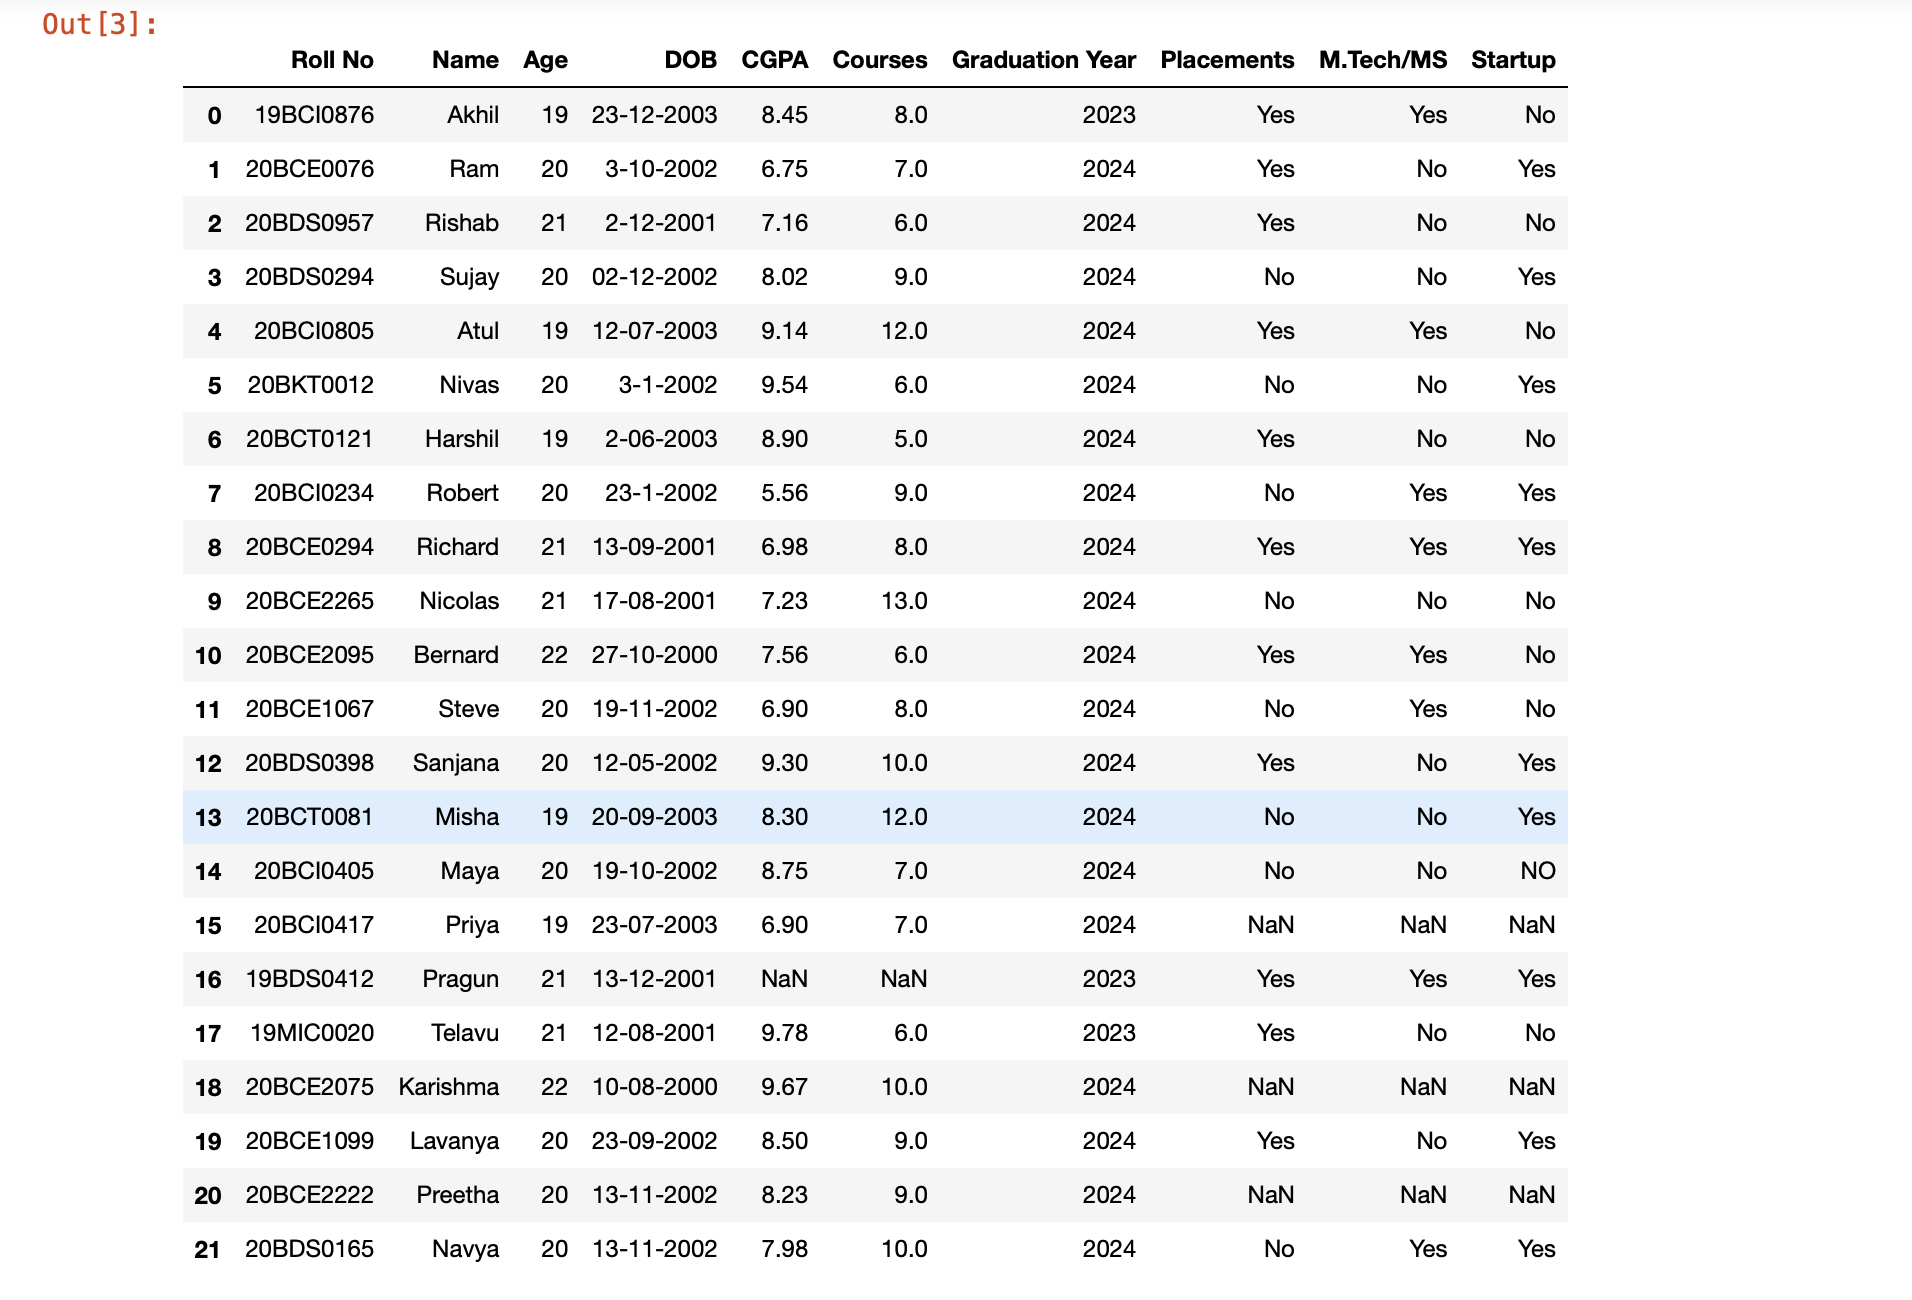
\includegraphics[scale=0.6]{images/1.png}
	
	\section{Data Pre-Processing}
	\begin{enumerate}
		\item I used Indexing Order to identify each Student name.
	\end{enumerate}
	
	\subsection{I want to predict the guy/girl will be placed or not }
	\begin{enumerate}
		\item The attributes are Age, CGPA, Courses, GradYear
		\item The predictor Placements
	\end{enumerate}
	
	\begin{lstlisting}[language=Java]
		
		data = data.drop(["Roll No","Name","DOB","M.Tech/MS","Startup"],axis=1)
		data = data.dropna(axis=0)
		data.isnull().sum()
		X = data.iloc[:,:4]
		y = data.iloc[:,4:]
		# Target Variable
		y = y["Placements"].apply(lambda x : 1 if x=='Yes' else 0)
		
		
		
	\end{lstlisting}
	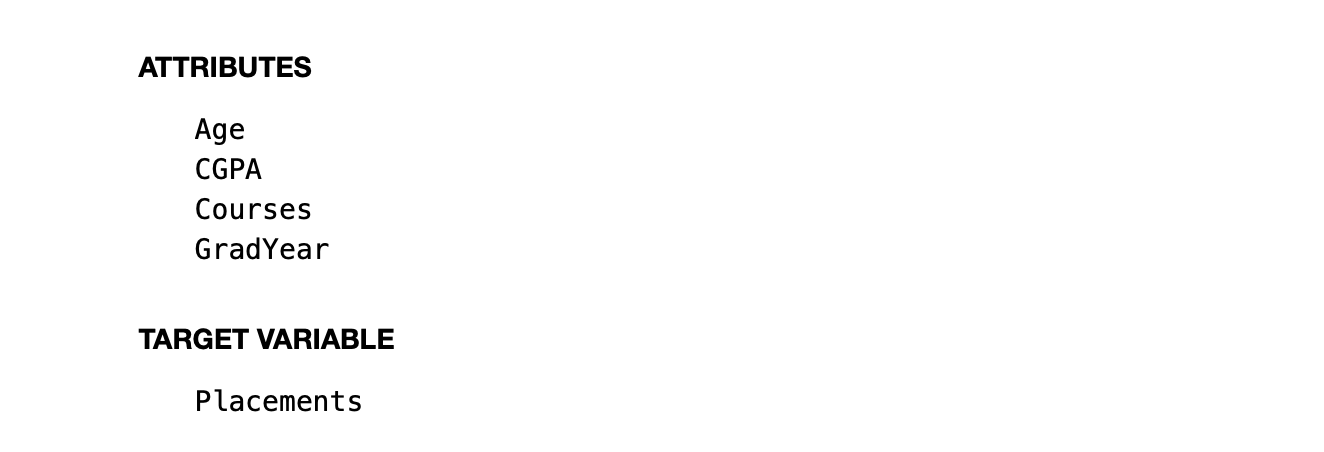
\includegraphics[scale=0.6]{images/2.png}\\\\\\
	
	
	\section{Decision Tree Classifier by SKLEARN}
	\begin{lstlisting}[language=Python]
		X_train, X_test, y_train, y_test = train_test_split(X, y, random_state = 20, train_size = 0.7)
		clf = DecisionTreeClassifier()
		clf.fit(X_train, y_train)
		y_pred_test =  clf.predict(X_test)
		y_pred_train=clf.predict(X_train)
		
		
		#pre-pruning
		
		
		
		max_depth = []
		acc = []
		for i in range(1,30):
		dt_classifier = DecisionTreeClassifier(max_depth=i, random_state = 30)
		dt_classifier.fit(X_train, y_train)
		pred = dt_classifier.predict(X_test)
		acc.append(accuracy_score(y_test, pred))
		max_depth.append(i)
		print(acc)
		print(max(acc))
		
		depth = acc.index(max(acc)) + 1
		dt_classifier = DecisionTreeClassifier(max_depth=depth, random_state = 20)
		dt_classifier.fit(X_train, y_train)
		pred = dt_classifier.predict(X_test)
		
		#pred
		accuracy_score(y_test, pred)
		
		
		
		#params = {'max_leaf_nodes': list(range(2, 100)), 'min_samples_split': [2, 3, 4]}
		params = {"criterion": ["gini", "entropy"],
			"min_samples_split": [2, 5],
			"max_depth": [7],
			"min_samples_leaf": [1, 3, 5, 7],
			"max_leaf_nodes": [None, 3, 5, 7],
		}
		grid_search_cv = GridSearchCV(DecisionTreeClassifier(random_state=20), params,cv=3, scoring='accuracy')
		
		grid_search_cv.fit(X_train, y_train)
		
		
		# By default, GridSearchCV trains the best model found on the whole training set (you can change this by setting refit=False), 
		#so we don't need to do it again. We can simply evaluate the model's accuracy:
		y_pred = grid_search_cv.predict(X_test)
		accuracy_score(y_test, y_pred)
		
	\end{lstlisting}
	
	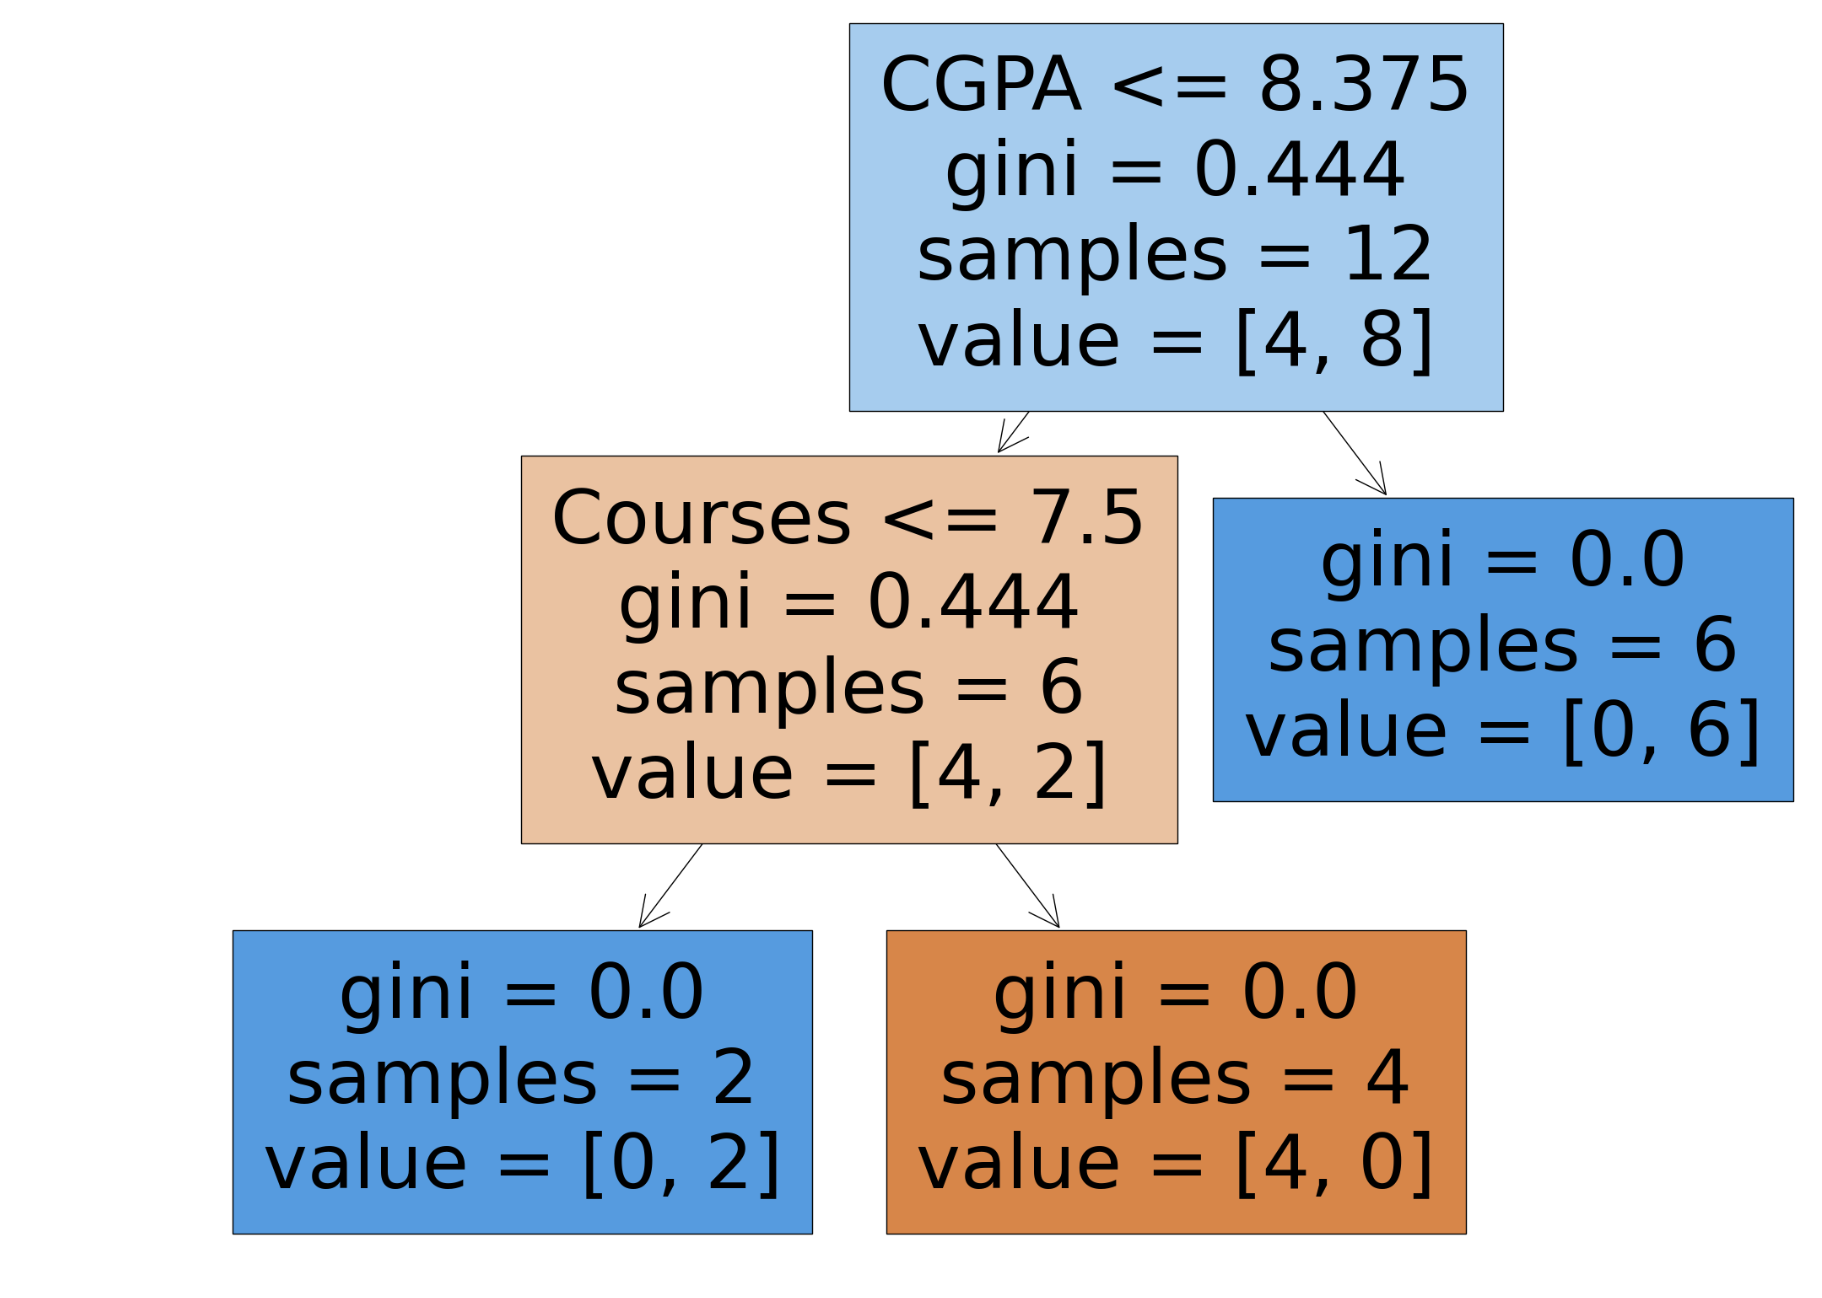
\includegraphics[scale=0.4]{images/3.png}\\\\
	\\\\
	
	
	\section{Neural Networks}
	\begin{lstlisting}[language= Python]
	class NeuralNetwork:
	
	# constructs the neural network
	def __init__(self, nn_inputs, nn_outputs, nn_epochs):
	self.inputs = nn_inputs
	self.outputs = nn_outputs
	self.epochs = nn_epochs
	self.hidden = 0
	self.error = 0
	
	# seeds e random number generator
	np.random.seed(1)
	# gets synaptic weights from -1 ro 1
	self.synaptic_weights = 2 * np.random.random((3, 1)) - 1
	self.error_history = []
	self.epoch_list = []
	
	# Using the sigmoid function
	def sigmoid(self, x, derivative=False):
	if not derivative:
	return 1 / (1 + np.exp(-x))
	else:
	# returns derivative of sigmoid function
	return x * (1 - x)
	
	# data will flow through the neural network.
	def feed_forward(self):
	self.hidden = self.sigmoid(np.dot(self.inputs, self.synaptic_weights))
	
	# going backwards through the network to update weights
	def backpropagation(self):
	self.error = self.outputs - self.hidden
	delta = self.error * self.sigmoid(self.hidden, derivative=True)
	self.synaptic_weights += np.dot(self.inputs.T, delta)
	
	# trains model to make accurate predictions while continually adjusting weights
	def train(self):
	for epoch in range(self.epochs):
	# go forward and produce an output
	self.feed_forward()
	# go back through the network and make corrections based on the output
	self.backpropagation()
	
	# keep track of input data
	self.error_history.append(np.average(np.abs(self.error)))
	self.epoch_list.append(epoch)
	
	# function to predict output on new and unseen input data
	def predict(self, new_input):
	prediction = self.sigmoid(np.dot(new_input, self.synaptic_weights))
	return prediction
	
	
	def run(run_inputs, run_outputs, run_iterations, run_new_inputs):
	# initializes neural network class
	neural_network = NeuralNetwork(run_inputs, run_outputs, run_iterations)
	
	# trains network
	neural_network.train()
	
	# print the predictions for new inputs
	for i in range(len(run_new_inputs)):
	print(run_new_inputs[i])
	print(neural_network.predict(run_new_inputs[i]), ' - Correct: ', run_new_inputs[i][0])
	
	# plot the error over the entire training duration
	plt.figure(figsize=(15, 5))
	plt.plot(neural_network.epoch_list, neural_network.error_history)
	plt.xlabel('Epoch')
	plt.ylabel('Error')
	plt.show()
	
	
	# provides all possible datasets
	def data():
	data_input = []
	
	for i1 in range(0, 2):
		for i2 in range(0, 2):
			for i3 in range(0, 2):
				data_input.append([i1, i2, i3])
		return data_input
	
	
	# gets the outputs for a set of inputs
	def get_outputs(get_outputs_inputs):
		get_outputs_outputs = []
	for i in range(0, len(get_outputs_inputs)):
		get_outputs_outputs.append([get_outputs_inputs[i][0]])
	return get_outputs_outputs
	
	
	\end{lstlisting}
	
	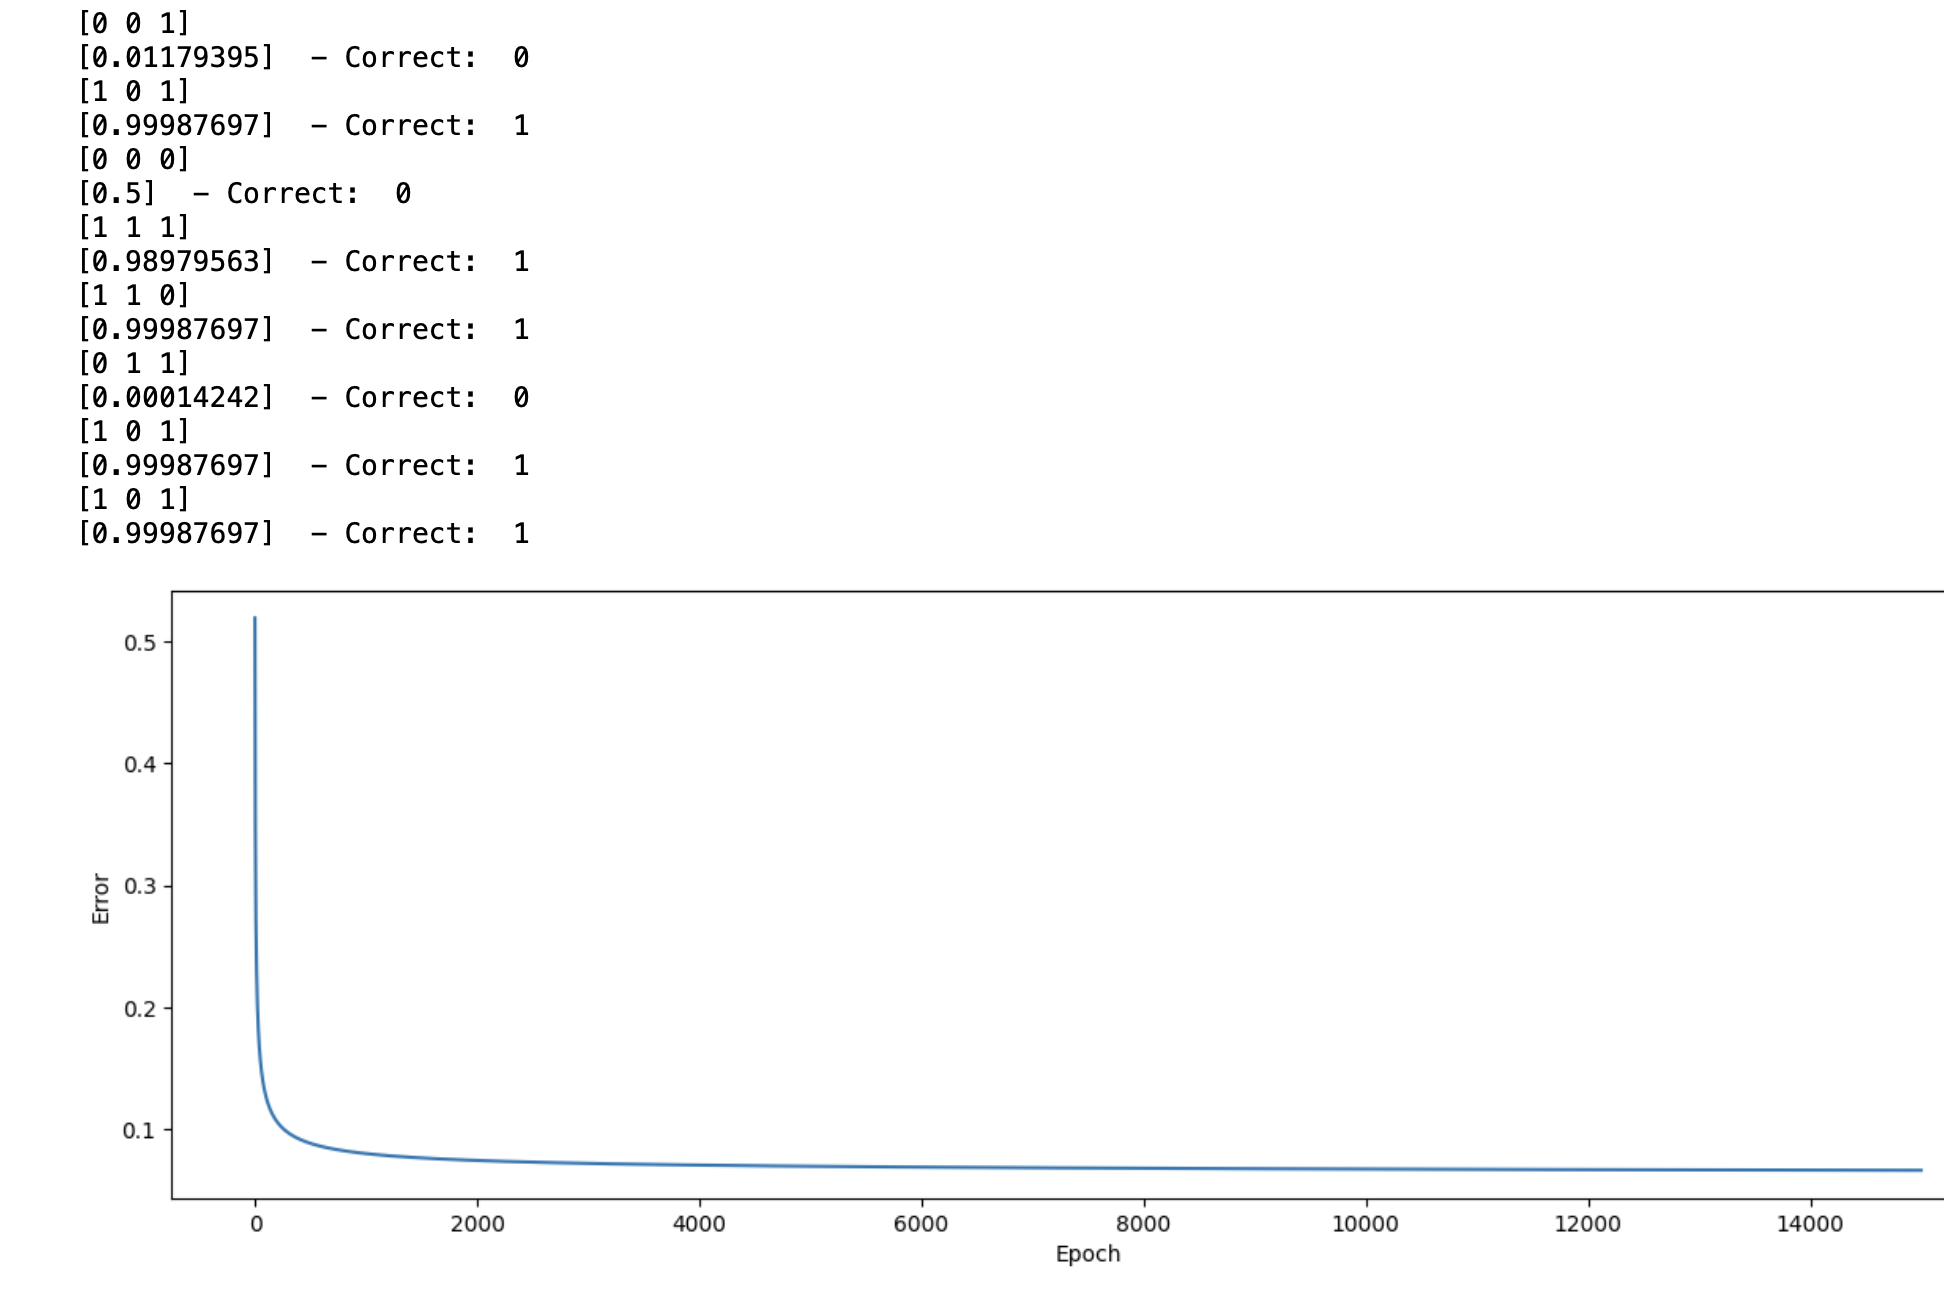
\includegraphics[scale=0.5]{images/4.png}\\\\

	
	
	\section{K Nearest Neighbors}
	
	\begin{lstlisting}[language=Python]
		from math import sqrt
		class KNN():
		def __init__(self,k):
		self.k=k
		print(self.k)
		
		def fit(self,X_train,y_train):
		self.x_train=X_train
		self.y_train=y_train
		
		def calculate_euclidean(self,sample1,sample2):
		distance=0.0
	
		
		def nearest_neighbors(self,test_sample):
		distances=[]#calculate distances from a test sample to every sample in a training set
		for i in range(len(self.x_train)):
		distances.append((self.y_train[i],self.calculate_euclidean(self.x_train[i],test_sample)))
		distances.sort(key=lambda x:x[1])#sort in ascending order, based on a distance value
		neighbors=[]
		for i in range(self.k): #get first k samples
		neighbors.append(distances[i][0])
		return neighbors
		
		def predict(self,test_set):
		predictions=[]
		test_set= np.array(test_set)
		for test_sample in test_set:
		neighbors=self.nearest_neighbors(test_sample)
		labels=[sample for sample in neighbors]
		prediction=max(labels,key=labels.count)
		predictions.append(prediction)
		return predictions
	\end{lstlisting}
	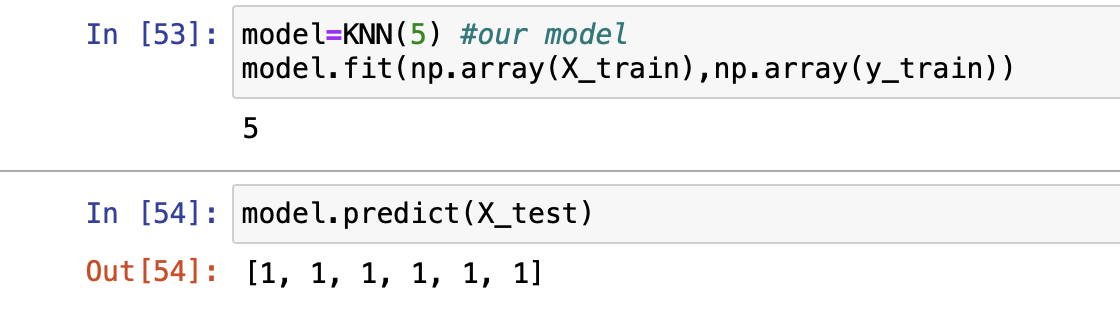
\includegraphics[scale=0.8]{images/5.png}
\end{document}